\section{Description de notre \textit{Clustering Interactif}}
\label{section:3.2-DESCRIPTION-THEORIQUE}

	Sur la base des intuitions que nous venons de détailler, nous proposons la méthode suivante dans le but d'assister la modélisation et l'annotation d'une collecte de données brutes en une base d'apprentissage nécessaire à l'entraînement d'un assistant conversationnel.
	
	%%%
	%%% Subsection 3.2.1. Description générale.
	%%%
	\subsection{Description générale}
	\label{section:3.2.1-DESCRIPTION-THEORIQUE-GENERALE}
	
		% Présentation succinte.
		\textbf{Notre méthode d'annotation}, que nous appelons \textguillemets{\texttt{Clustering Interactif}}, \textbf{repose sur l'alternance successive entre deux phases clefs} (voir \textsc{Figure~\ref{figure:3.2.1-DESCRIPTION-THEORIQUE-GENERALE}}) :
		\begin{itemize}
			\item[\(\bullet\)] une phase d'\textbf{annotation de contraintes}
			par un expert permettant de caractériser la similarité entre deux données suivant leur cas d'usage métier ;
			\item[\(\bullet\)] une phase de \textbf{segmentation automatique} des données
			par une machine sur la base de la proximité sémantique des données et des contraintes précédemment annotées.
		\end{itemize}
		
		% Objectif recherché
		L'objectif recherché en associant ces deux phases est de \textbf{créer un cercle vertueux pour améliorer itérativement la qualité de la base d'apprentissage} en cours de construction.
		En effet, à chaque itération, l'expert métier obtiendra une proposition de segmentation des données qu'il pourra affiner dans le but de corriger le fonctionnement de la machine et ainsi d'obtenir une segmentation plus pertinente à l'itération suivante.
		
		% Figure.
		\begin{figure}[!htb]
			\centering
			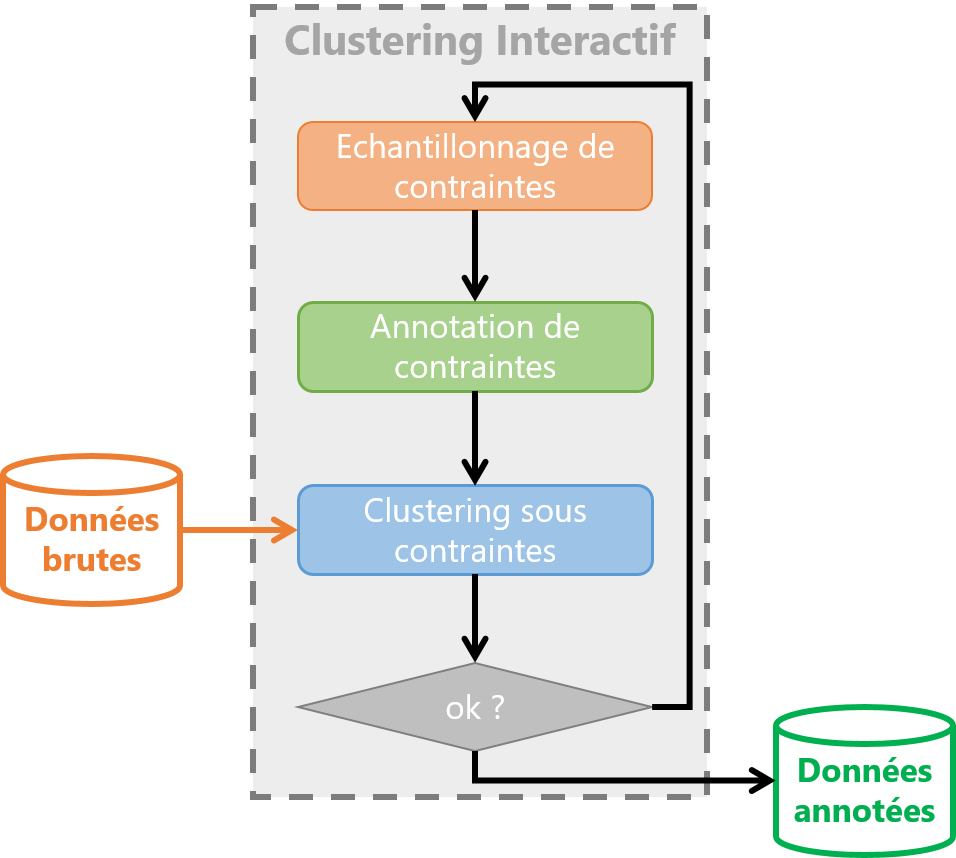
\includegraphics[width=0.95\textwidth]{figures/interactive-clustering-architecture-sequentielle}
			\caption{
				Schéma illustrant l'architecture du \texttt{Clustering Interactif}.
				La boucle principale enchaîne un échantillonnage de couples de données, une annotation de contraintes, et un \textit{clustering} sous contraintes.
			}
			\label{figure:3.2.1-DESCRIPTION-THEORIQUE-GENERALE}
		\end{figure}
	
	
	%%%
	%%% Subsection 3.2.2. Description détaillée.
	%%%
	\subsection{Description détaillée}
	\label{section:3.2.2-DESCRIPTION-THEORIQUE-DETAILLEE}
	
		% Pseudo code.
		L'\textsc{Algorithme~\ref{algorithm:3.2-CLUSTERING-INTERACTIF}} décrit formellement notre proposition de \texttt{Clustering Interactif} que nous détaillons ci-dessous.
		\begin{algorithm}
			\KwData{données non segmentées}
			\KwIn{budget à disposition}
			%
			\textbf{initialisation}: créer une liste vide de contraintes \;
			\textit{optionnel}: évaluer les hyperparamètres de la segmentation automatique \;
			\textbf{segmentation initial}: regrouper les données par similarité \;
			\Repeat{segmentation satisfaisante OU budget épuisé}{
				\textit{optionnel}: évaluer les hyperparamètres de l'échantillonnage \;
				\textbf{échantillonnage}: sélectionner une partie de la segmentation à corriger \;
				\textbf{annotation}: corriger la segmentation en ajoutant des contraintes sur l'échantillon \;
				\textit{optionnel}: réévaluer les hyperparamètres de la segmentation automatique \;
				\textbf{segmentation}: regrouper les données par similarité avec les contraintes \;
				\textbf{validation}: estimer la pertinence et la stabilité de la segmentation \;
				\textbf{coûts}: estimer le budget restant et les coûts restants à investir \;
			}
			\textbf{interprétation}: trier et nommer les clusters pour les exploiter \;
			%
			\KwResult{données segmentées (i.e. base d'apprentissage)}
			%
			\caption{\textit{
				Description en pseudo-code de la méthode d'annotation proposée employant le \texttt{Clustering Interactif}.
			}}
			\label{algorithm:3.2-CLUSTERING-INTERACTIF}
		\end{algorithm}
		
		% Description de l'initialisation.
		Pour l'\textbf{initialisation} de la méthode (cf. \textsc{Algorithme~\ref{algorithm:3.2-CLUSTERING-INTERACTIF}}, \textit{lignes 1 à 3}), nous définissons une liste vide de contraintes : tout au long du processus, nous y ajoutons les contraintes annotées par l'expert grâce à ses connaissances métiers (nous entrerons en détails en décrivant la phase d'annotation).
		Il faut aussi une première segmentation des données par la machine : celle-ci se réalise par l'exécution d'un algorithme de \textit{clustering}.
		Nous estimons qu'il n'est pas du ressort de l'expert métier de choisir l'algorithme de \textit{clustering} ni de régler ses hyperparamètres.
		Ces derniers pourront être déterminés par un \textit{data scientist} en fonction du problème à traiter.
		Il est à noter que cette première segmentation des données est réalisée sans bénéficier de la connaissance de l'expert, il est donc peu probable que le résultat soit pertinent à ce stade.
		
		% Description de l'échantillonnage.
		Nous entrons dans le coeur de la boucle itérative par la phase d'\textbf{échantillonnage} (cf. \textsc{Algorithme~\ref{algorithm:3.2-CLUSTERING-INTERACTIF}}, \textit{lignes 5 et 6}).
		Comme mentionné au préalable, savoir quelles contraintes ajouter pour corriger efficacement le \textit{clustering} est un problème NP-difficile (le nombre de possibilités croît proportionnellement au carré du nombre de données).
		De plus, l'intervention d'experts est chiffrée et représente en général une partie des coûts à investir dans un projet (voir \textsc{Section~\ref{section:2.3.2.C-DEFIS-ANNOTATION-ASPECT-COMPLEXITE-COUTS}}).
		Il est donc inconcevable de laisser un expert métier annoter des contraintes "\textit{seul}" et "\textit{au hasard}".
		Ainsi, pour optimiser ses interventions, il convient de déterminer là où l'expert aura le plus d'impact lors de sa transmission de connaissances.
		C'est pourquoi la phase d'échantillonnage est primordiale dans la méthode proposée : nous proposons d'y sélectionner des couples de données sur la base de leur similarité, de leur segmentation ou encore de leurs relations avec d'autres données déjà liées par des contraintes.
		
		% Description de l'annotation.
		Sur la base de cet échantillon, l'expert peut entamer son étape d'\textbf{annotation de contraintes} (cf. \textsc{Algorithme~\ref{algorithm:3.2-CLUSTERING-INTERACTIF}}, \textit{ligne 7}).
		Pour alléger la charge d'annotation, nous avons décidé de discriminer les données de l'échantillon par des contraintes binaires simples : \texttt{MUST-LINK} et \texttt{CANNOT-LINK}.
		Ces contraintes représentent respectivement la similitude ou la différence entre deux données, et seront utilisées pour regrouper ou séparer certaines données dans la prochaine segmentation.
		En fonction de l'orientation du projet et afin de rester au plus proche des compétences réelles de l'expert, la formulation de l'énoncé d'annotation doit être judicieusement définie : par exemple, les contraintes peuvent représenter une similitude
		sur la thématique concernée \footnote{
			Exemples de thématiques : \textit{crédit} vs. \textit{assurance} ; \textit{sport} vs. \textit{culture}, ...
		}, sur l'action désirée \footnote{
			Exemples d'actions : \textit{souscrire} vs. \textit{résilier} ; \textit{activer} vs. \textit{désactiver} ; \textit{s'informer} vs. \textit{réaliser}, ...
		}, ou encore sur le besoin de l'utilisateur \footnote{
			Exemple de besoins : \textit{souscrire un crédit} vs. \textit{souscrire une assurance} ; \textit{s'informer en sport} vs. \textit{s'informer en culture}, ...
		}.
		Nous noterons que des incohérences peuvent s'introduire, ayant pour conclusions de devoir à la fois considérer comme similaires et différentes deux données : ces incohérences peuvent être détectées grâce aux propriétés de transitivité des contraintes (voir la gestion des conflits en \textsc{Annexe~\ref{annex:C.1.2-DESCRIPTION-IMPLEMENTATION-INTERACTIVE-CLUSTERING-GESTION-DES-CONTRAINTES}}).
		
		% Description du \textit{clustering}.
		Pour finir, la dernière phase de cette boucle est composée d'une nouvelle \textbf{segmentation} des données (cf. \textsc{Algorithme~\ref{algorithm:3.2-CLUSTERING-INTERACTIF}}, \textit{lignes 8 et 9}).
		Cette segmentation devra respecter les contraintes préalablement définies par l'expert, nous nous tournons donc vers l'utilisation d'un \textit{clustering} sous contraintes.
		Au fur et à mesure des itérations, de plus en plus de contraintes seront ajoutées pour corriger le \textit{clustering}.
		Ainsi, au bout d'un certain nombre d'itérations, la segmentation des données reflétera la vision que l'expert aura voulu transmettre.
		Comme précédemment, nous estimons qu'il n'est pas du ressort de l'expert métier de choisir l'algorithme de \textit{clustering} ni de régler ses hyperparamètres.
		Ces derniers pourront être déterminés par un \textit{data scientist} en fonction du problème à traiter, de l'itération en cours et des contraintes disponibles.
		
		% Description de l'évaluation.
		Comme la méthode est itérative, il faut pouvoir estimer des \textbf{cas d'arrêt} (cf. \textsc{Algorithme~\ref{algorithm:3.2-CLUSTERING-INTERACTIF}}, \textit{lignes 10 à 12}).
		Le cas d'arrêt le plus évident n'est pas technique mais relatif aux coûts investis dans l'opération : si le projet n'a plus de budget dédié à l'annotation, il faudra créer la base d'apprentissage avec le résultat à disposition, quel que soit la pertinence de la segmentation obtenue sur les données.
		Ce cas d'arrêt par défaut peut malheureusement être synonyme d'échec pour le projet si les résultats sont inexploitables.
		D'autres cas d'arrêts peuvent être envisagés en fonction de la qualité ou de la pertinence de la segmentation.
		D'une part, nous pouvons comparer l'évolution de la segmentation des données : si les segmentations sont similaires sur plusieurs itérations, il est possible que la modélisation atteigne un optimum local.
		D'autre part, nous pouvons aussi comparer l'évolution de l'accord entre la segmentation obtenue et l'annotation de l'expert : en effet, si l'expert ne contredit plus la répartition proposée des données, il est probable que sa vision et la vision de la machine aient convergé.
		Dans les deux cas, l'analyse de l'expert métier reste nécessaire pour valider si la modélisation des données est pertinente ou si elle comporte encore des incohérences à corriger.

		% Description de l'évaluation.
		Lorsque la boucle itérative est finie, nous avons à disposition une segmentation des données qui a été corrigée par un expert et qui reflète ses connaissances métier.
		La dernière étape consiste alors à \textbf{interpréter} ces \textit{clusters} pour pouvoir les exploiter (cf. \textsc{Algorithme~\ref{algorithm:3.2-CLUSTERING-INTERACTIF}}, \textit{ligne 13}).
		Cela commence par leur attribuer un nom au lieu de leur identifiant technique, de les définir en les rapprochant d'un cas d'usage métier, et éventuellement de les raffiner manuellement en supprimant certaines données aberrantes.
		
		% Exemple abstrait.
		\begin{leftBarExamples}
			La \textsc{Figure~\ref{figure:3.2.2-DESCRIPTION-THEORIQUE-DETAILLEE-EXEMPLE}} déroule l'initialisation et la première itération de la méthode sur un exemple fictif.
			Nous pouvons constater qu'entre les images \textbf{(2)} et \textbf{(5)}, la segmentation des données a évolué grâce à l'introduction de contraintes.
		
			\begin{figure}[H]
				\centering
				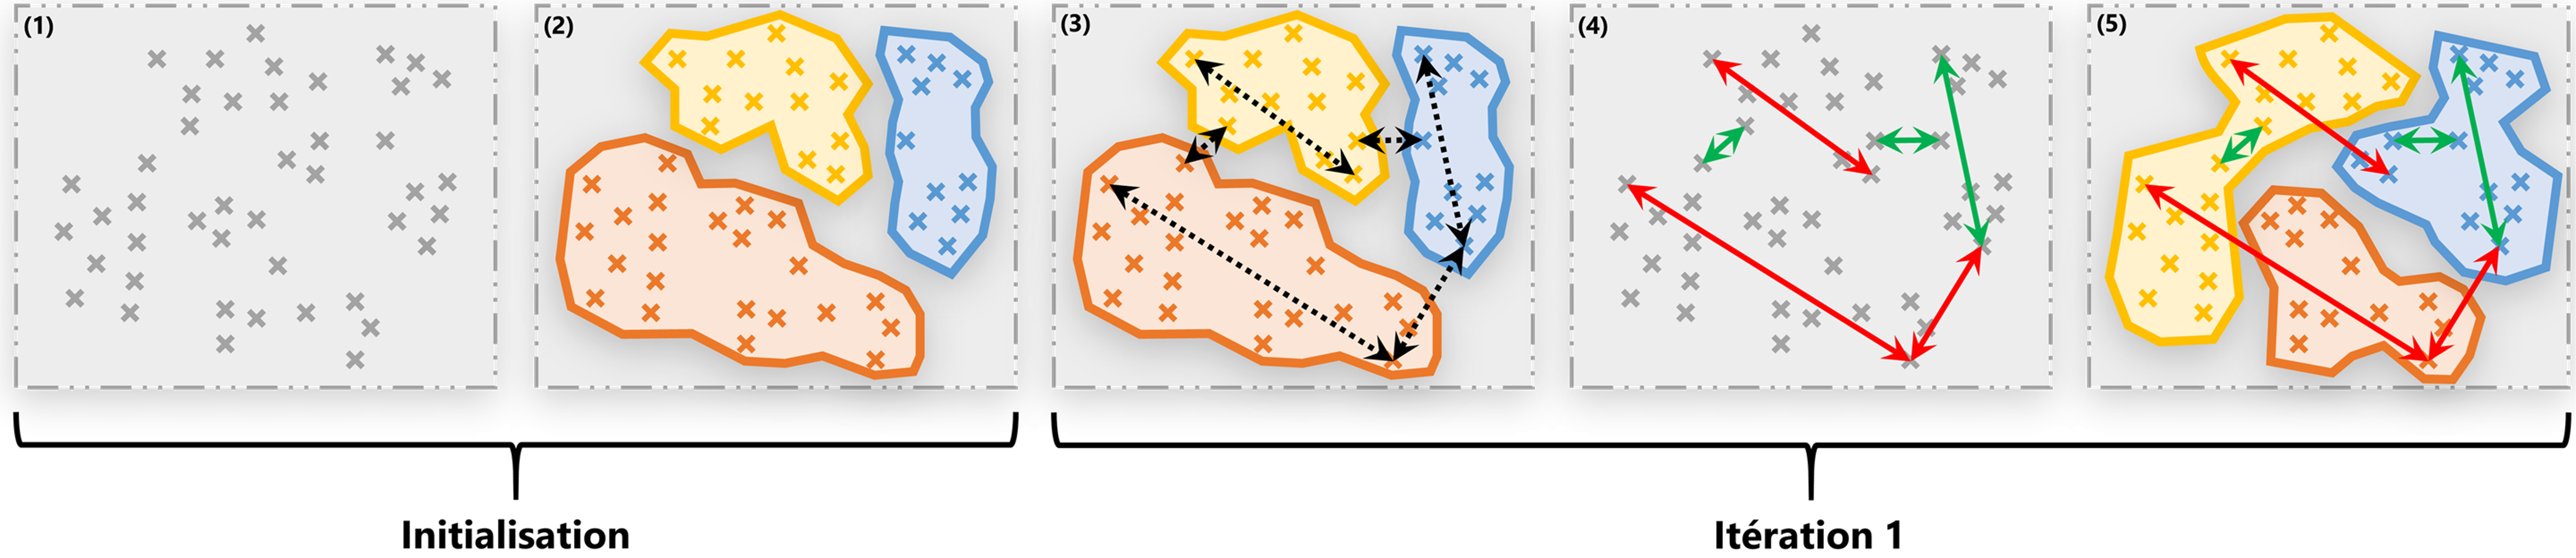
\includegraphics[width=0.95\textwidth]{figures/example-iteration-clustering-interatif}
				\caption{
					Exemple d'une itération de \texttt{Clustering Interactif}. \\
					Lors de l'initialisation,
					\textbf{(1)} correspond au jeu de données brut,
					et \textbf{(2)} correspond à une première segmentation des données en $3$ \textit{clusters}.
					Lors de l'itération $1$ :
					\textbf{(3)} correspond à un exemple d'échantillonnage de $6$ contraintes représentées par les flèches en pointillé,
					\textbf{(4)} correspond à la caractérisation de ces $6$ contraintes par des liens \texttt{MUST-LINK} en vert et \texttt{CANNOT-LINK} en rouge,
					et \textbf{(5)} correspond à la nouvelle segmentation des données en $3$ \textit{clusters} respectant les $6$ contraintes annotées.
					La prochaine itération se poursuivra par un nouvel échantillonnage de contraintes.
				}
				\label{figure:3.2.2-DESCRIPTION-THEORIQUE-DETAILLEE-EXEMPLE}
			\end{figure}
		\end{leftBarExamples}
	
	
	%%%
	%%% Subsection 3.2.3. Descriptions techniques et implémentation.
	%%%
	\subsection{Descriptions techniques et implémentation}
	\label{section:3.2.3-DESCRIPTION-TECHNIQUE-IMPLEMENTATION}
	
		% Généralités.
		Au cours de ce doctorat, nous avons réalisé un ensemble d'implémentations en \texttt{Python} afin de mettre en oeuvre notre méthodologie de \textit{Clustering Interactif}.
		Celle-ci est répartie en trois librairies :
		\begin{enumerate}
			% cognitivefactory-interactive-clustering
			\item \texttt{cognitivefactory-interactive-clustering} \footnote{
				\url{https://pypi.org/project/cognitivefactory-interactive-clustering/}
			} (\cite{schild:2022:cognitivefactory-interactiveclustering}), regroupant les gestions de données et des contraintes, les algorithmes de \textit{clustering} et d'échantillonnage ;
			% cognitivefactory-interactive-clustering-gui
			\item \texttt{cognitivefactory-interactive-clustering-gui} \footnote{
				\url{https://pypi.org/project/cognitivefactory-interactive-clustering-gui/}
			} (\cite{schild-etal:2022:cognitivefactory-interactiveclusteringgui}), intégrant la logique de la méthodologie dans une application web ;
			% cognitivefactory-features-maximization-metric
			\item \texttt{cognitivefactory-features-maximization-metric} \footnote{
				\url{https://pypi.org/project/cognitivefactory-features-maximization-metric/}
			} (\cite{schild:2023:cognitivefactory-featuresmaximizationmetric}), disposant d'une méthode de sélection des patterns linguistiques caractéristiques d'un jeu de données labellisées, permettant ainsi d'analyser la pertinence d'un résultat de \textit{clustering}.
		\end{enumerate}
		
		
		% Exemple de visuels de l'application.
		\begin{leftBarExamples}
			La \textsc{Figure~\ref{figure:3.2.3-DESCRIPTION-TECHNIQUE-IMPLEMENTATION-EXEMPLE}} représente une capture d'écran de la page d'annotation de contraintes de l'application web intégrant notre méthodologie de \texttt{Clustering Interactif}.
			
			% Capture d'écran: annotation.
			\begin{figure}[H]
				\centering
				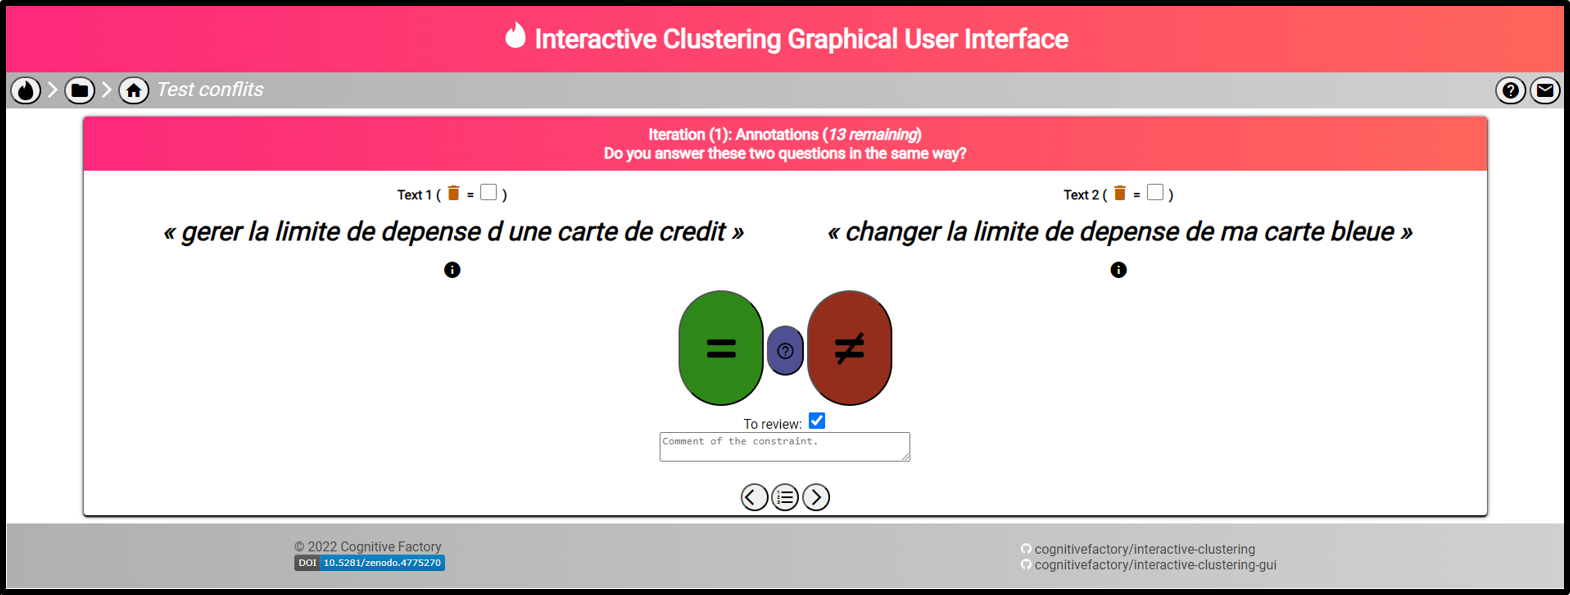
\includegraphics[width=0.95\textwidth]{figures/interactive-clustering-application-annotation-0small}
				\caption{
					Capture d'écran de l'application web implémentant notre méthodologie de \texttt{Clustering Interactif} : \textbf{page d'annotation d'une contrainte}.
					Parmi les éléments importants, nous retrouvons les deux textes à annoter (disposés à gauche et droite de l'écran) et les boutons d'annotation (bouton vert pour un \texttt{MUST-LINK}, bouton rouge pour un \texttt{CANNOT-LINK}.
					Les autres fonctionnalités sont détaillées en \textsc{Annexe~\ref{annex:C.2-DESCRIPTION-IMPLEMENTATION-INTERACTIVE-CLUSTERING-GUI}}.
				}
				\label{figure:3.2.3-DESCRIPTION-TECHNIQUE-IMPLEMENTATION-EXEMPLE}
			\end{figure}
		\end{leftBarExamples}
		
		% Information : voir en annexe.
		\begin{leftBarInformation}
			Ces implémentations sont présentées dans l'\textsc{Annexe~\ref{annex:C-ANNEXE-IMPLEMENTATIONS}}.
			L'ensemble des détails techniques et des explications sur les choix d'implémentation y sont décrits.
		\end{leftBarInformation}